\documentclass[10pt,journal]{IEEEtran}
\usepackage[letterpaper,top=1in,bottom=1in,left=.7in,right=.7in,columnsep=.2in]{geometry}
\usepackage{amsmath,amssymb,graphicx,booktabs,array,fontspec,placeins,balance}
\usepackage[hidelinks]{hyperref}
\setmainfont{Times New Roman}
\newtheorem{proposition}{Proposition}
\newtheorem{corollary}{Corollary}
\newcommand{\norm}[1]{\lVert#1\rVert}
\newcommand{\um}{\,\mu\mathrm{rad}}
\def\FrontierRows{
R1 below & UAD & 221/600 & 221/600 & 0.000 & 3.084 & 6 & 0.646 \\
R1 below & Fixed guard & 0/600 & 0/600 & 0.000 & 0.000 & 0 & -- \\
R1 middle & UAD & 600/600 & 594/600 & 0.000 & 8.331 & 26 & 0.658 \\
R1 middle & Fixed guard & 0/600 & 0/600 & 0.000 & 0.000 & 0 & -- \\
R1 above & UAD & 600/600 & 594/600 & 0.000 & 8.331 & 26 & 0.666 \\
R1 above & Fixed guard & 239/600 & 233/600 & 0.000 & 3.319 & 6 & 0.924 \\
R2 below & UAD & 0/600 & 0/600 & 0.000 & 0.000 & 0 & -- \\
R2 below & Fixed guard & 28/600 & 28/600 & 0.000 & 0.393 & 0 & 1.036 \\
R2 middle & UAD & 0/600 & 0/600 & 0.000 & 0.000 & 0 & -- \\
R2 middle & Fixed guard & 41/600 & 41/600 & 0.000 & 0.565 & 0 & 1.048 \\
R2 above & UAD & 0/600 & 0/600 & 0.000 & 0.000 & 0 & -- \\
R2 above & Fixed guard & 0/600 & 0/600 & 0.000 & 0.000 & 0 & -- \\
}

\def\EvidenceRows{
V4 & within-premise & 0 & 0 \\
V4 & out-of-model & 557 & 100 \\
V4 & unverified & 1564 & 0 \\
V5 & within-premise & 402 & 0 \\
V5 & out-of-model & 968 & 350 \\
V5 & unverified & 0 & 0 \\
V6 & within-premise & 1421 & 0 \\
V6 & out-of-model & 0 & 0 \\
V6 & unverified & 0 & 0 \\
}

\graphicspath{{results/}}
\raggedbottom
\begin{document}
\title{Conditional Probe Authorization for Optical Diagnosis With Finite-Model Actuator Bounds}
\author{}
\maketitle
\begin{abstract}
Diagnostic excitation can interrupt a working optical link while distinguishing pointing loss from attenuation. A fixed angular guard is easy to deploy, but its adequacy is not established merely by successful simulations. This paper formulates conditional probe authorization using a reference-relative optical-power inequality, a simultaneous sensor event valid at an observation-selected start, and an explicitly finite actuator-model enclosure. It separates probe service, estimator uncertainty, diagnostic acceptance and recovery. Earlier evaluations produced identical trajectories for the certified and fixed-guard selectors in 2,800 paired cases. A development-guided admission-frontier study now tests both disagreement directions and surrounding controls in 7,200 new runs. In a low-noise, nondeclining-gain region, the certificate admits 600 probes and accepts 594 parameter fits, versus no admitted probes for a fixed 2-microradian guard; both methods have zero sampled outage. In the reverse region, the guard admits probes refused by the certificate without observed outage. Thus the observed benefit is diagnostic access in a restricted regime, not universal recovery improvement or proof that guard admissions are unsafe. Separate numerical replay checks 5,040,000 recorded actuator steps. Historical records are classified as within-premise, out-of-model or unverified according to available evidence. A supervisory interface refuses missing or expired contracts and never equates probe authorization with a correct diagnosis. Physical calibration, continuous-parameter robustness and independent external review remain absent.
\end{abstract}
\begin{IEEEkeywords}Optical diagnosis, supervisory control, active probing, conditional certification, measurement uncertainty.\end{IEEEkeywords}

\section{Problem and Contribution}
Scalar optical power cannot by itself distinguish a pointing offset from reduced optical gain. Moving the beam can supply diagnostic information, but that movement can degrade an otherwise usable communication link. The operational question examined here is whether a supervisory layer can authorize a finite diagnostic probe under a stated sampled-outage budget. It is separate from whether the resulting estimate is accurate, whether an acceptance test is reliable, and whether a subsequent correction recovers service.

Optical acquisition and extremum-seeking alignment are established \cite{guelman,es}. Chance-constrained active diagnosis already allocates state-constraint risk \cite{guo}; uncertain nonlinear guaranteed diagnosis already uses reachability verification \cite{massa}. Safety-filtered extremum seeking provides practical semiglobal statements for measured unknown barrier functions \cite{safees}. Link-margin-aware optical scanning is also prior art \cite{yan}. This work claims neither the invention of safe active diagnosis nor the absence of guarantees in those differently formulated methods.

The precise mathematical property is conditional: if the true actuator belongs to a declared finite set, the optical window satisfies fixed-offset/divergence and gain hypotheses, and a stipulated sensor event holds, actual sampled probe-window outage is bounded by a computed count. The sensor event has probability at least $1-\delta$ under its marginal-tail model, including an observation-selected start. Norm inequalities, simultaneous events and finite impulse enclosures are known tools; the present result is a specialized optical deployment statement. Absolute priority over every close optical method remains unconfirmed.

The practical question is deliberately narrower than recovery superiority. In the prior revision, UAD and a fixed-$2\um$-guard selector had identical power, angle and probe histories in all 2,800 paired cases. We retain that result and investigate admission boundaries where the methods can differ, using both directions and controls. We also specify what a supervisor requires and how it should refuse a request when its supporting evidence is unavailable. The interface is evaluated with simulation contracts in shadow mode; no physical deployment is claimed.

\section{Model and Four Distinct Properties}
The reused terminal model \cite{source} has two angular axes. Each has angle $q$, rate $v$, delivered torque $a$ and integral state $I$:
\begin{align}
\dot q&=\operatorname{clip}(v),&J_a\dot v&=a-dv,\nonumber\\
\tau_a\dot a&=u_c-a,&\dot I&=q_m-r.
\end{align}
The implementation includes rate clamping and anti-windup. A fixed nominal PID computes
\begin{align}
u_{\rm raw}&=-J_0k_p(q_m-r)+(d-J_0k_d)v_m-J_0k_iI,\nonumber\\
u_c&=\operatorname{clip}_{u_{\max}}(u_{\rm raw}).
\end{align}
Held-input RK4 advances the model every $\Delta t$. True $J_a,\tau_a$ can differ from nominal controller values. Received power is
\begin{equation}
p=p_0(\alpha)g\exp[-2\norm{q+b}^2/\alpha^2],
\label{eq:optical}
\end{equation}
with $p_0=P_t\eta_o[1-\exp(-2r_a^2/(L^2\alpha^2))]$. Service requires $p\geq p_{\min}$.

\begin{table}[t]
\caption{Declared simulation values, not hardware calibration.}
\centering\footnotesize
\begin{tabular}{@{}p{.43\columnwidth}p{.51\columnwidth}@{}}\toprule
Quantity & Assumed value\\\midrule
Range / aperture diameter & 800 km / 0.10 m\\
Transmit power / efficiency & 0.5 W / 0.4\\
Divergence / declared interval & $20\um$ / $[18,22]\um$\\
Aligned power / sensitivity & $3.9062~\mu$W / $1.5~\mu$W\\
$J_0,d,\tau_0$ & 0.002 kg m$^2$, 0.004 N m s/rad, 0.08 s\\
$k_p,k_d,k_i$ & 64 s$^{-2}$, 14 s$^{-1}$, 8 s$^{-3}$\\
Torque / rate limit & $2~\mu$N m / $120\um$/s\\
Nominal encoder / power std. dev. & $0.08\um$ / 0.008 relative\\
Step / mission duration & 0.02 s / 14 s\\
Actual finite model set & $J_a/J_0\in\{.8,1,1.25\}$; $\tau_a/\tau_0\in\{1,1.5\}$\\
Offset prior / maximum gain & $30\um$ / 1.05\\
Working-link outage budget & 0 s, sampled probe window only\\\bottomrule
\end{tabular}
\label{tab:model}
\end{table}

The measurement model is $q_m=q+\sigma_qZ_q$, $v_m=v+2\sigma_qZ_v$, and $p_m=\max\{0,p(1+\sigma_p Z_p)\}$. Five scalar standardized disturbances are stipulated marginal standard Gaussian. Their scales, the optics and actual actuator model are assumptions requiring external evidence in deployment. Hardware reviews and pointing-budget studies motivate considering uncertainty but do not calibrate this assumed unit \cite{actuators,baeck,nasa}. Receiver-side pointing, orbital geometry, queues and network routing are omitted.

\begin{table}[t]
\caption{Properties that must not be conflated.}
\footnotesize\centering
\begin{tabular}{@{}p{.25\columnwidth}p{.69\columnwidth}@{}}\toprule
Property & Actual statement / evidence\\\midrule
Probe service & Conditional bound on sampled outage during one authorized probe.\\
Offset estimate & Approximate GLS uncertainty; evaluate errors and coverage separately.\\
Diagnosis decision & Acceptance/rejection rule; no guaranteed correct fault label.\\
Recovery & Observed subsequent link availability; not implied by authorization or fit acceptance.\\\bottomrule
\end{tabular}
\label{tab:four}
\end{table}

For fixed exact angular regressors, projecting logarithmic power against affine temporal nuisance gives the familiar offset estimator. With $Q_i=q_i^T/\alpha$, $P$ the orthogonal nuisance projection and $F=Q^TPQ\succ0$, an exact-regressor Gaussian-log-noise calculation gives $C_b=\alpha^2\sigma^2F^{-1}/16$. Its enclosing 95\% radius uses $5.991464547\lambda_{\max}(C_b)$. Noisy regressors, multiplicative power noise and acceptance selection invalidate an exact transfer of this covariance. The implementation therefore labels feasible GLS covariance as approximate and reports accepted-fit coverage separately.

Bias illustrates the distinction structurally. If $q_m=q+\beta$, then $q+b=q_m+(b-\beta)$: the scalar-power model cannot distinguish true offset $b$ from shifted offset $b-\beta$. A small residual does not detect this ambiguity. In the preserved V5 affine-drift data, nominal UAD accepts 46/50 fits, with one confidence miss; with unmodeled $[2,-1]\um$ bias it accepts 39/50, all 39 outside their reported radius and above $1\um$ actual error. These are failures of diagnostic reliability, not consequences repaired by a service certificate.

\section{Conditional Optical Certificate}
\subsection{Line-by-line angular argument}
Let $e_0=q(t_0)+b$ and $d(t)=q(t_0+t)-q(t_0)$, with fixed $b,\alpha$ over the window and positive starting power. The exact identity is
\begin{equation}
\log\frac{p(t_0+t)}{p(t_0)}=\log\frac{g(t_0+t)}{g(t_0)}-\frac{2}{\alpha^2}(2e_0^Td+\norm d^2).
\end{equation}
It requires no zero starting angle.

\begin{proposition}
If $e_0\in\mathcal B(c,R)$ and $d\in\mathcal B(\bar d,r)$ with Euclidean radii in radians, then $2e_0^Td+\norm d^2\leq\overline D$, where
\begin{align}
\overline D={}&2c^T\bar d+2R\norm{\bar d}+\norm{\bar d}^2\nonumber\\
&+2(\norm{c+\bar d}+R)r+r^2.
\label{eq:general}
\end{align}
For $c=0$, its maximum is exactly
\begin{equation}
D_{\max}=2R(\norm{\bar d}+r)+(\norm{\bar d}+r)^2.
\label{eq:centered}
\end{equation}
\end{proposition}
\emph{Proof:} Put $e_0=c+u$, $d=\bar d+v$, $A=\norm{\bar d}$ and $B=\norm{c+\bar d}$. Exact expansion makes the slack in \eqref{eq:general}
\begin{align}
\overline D-(2e_0^Td+\norm d^2)
={}&2(RA-u^T\bar d)\nonumber\\
&+2(rB-(c+\bar d)^Tv)\nonumber\\
&+2(Rr-u^Tv)+(r^2-\norm v^2).
\end{align}
Every bracket is nonnegative by Cauchy--Schwarz and $\norm u\leq R$, $\norm v\leq r$. For $c=0$ and $A>0$, choose $u=R\bar d/A$, $v=r\bar d/A$. Both balls' boundaries are attained and the loss equals \eqref{eq:centered}. If $A=0$, use any common unit direction. The same construction permits $R=0$, $r=0$, or both zero. Noncentered sharpness is not claimed.\hfill$\square$

Every term in $\overline D$ has units radians squared. Changing all angles to microradians multiplies numerator and divergence squared by the same $10^{-12}$. With $p(t_0)\geq\underline p_0$, $\alpha\geq\alpha_{\min}$ and $\log(g/g(t_0))\geq-\ell t$,
\begin{equation}
\underline p(t)=\underline p_0\exp[-\ell t-2\max(\overline D(t),0)/\alpha_{\min}^2]
\label{eq:power}
\end{equation}
is a lower bound. For nonnegative loss the smallest divergence is conservative. For negative upper loss, dropping guaranteed improvement via $\max(\cdot,0)$ avoids reversing the divergence inequality. Angular sharpness does not imply global power tightness when gain, divergence and starting-power constraints are coupled.

A new exact-algebra audit checks the slack identity, the two-dimensional Gram determinant used by Cauchy--Schwarz, centered attainment including zero increment, and unit conversion. The preserved independent boundary search covers 1,200 cases and 9,600 direct power checks. This is a written proof with separate machine-checked identities and numerical corroboration, not an external human review or complete formally rounded theorem.

\subsection{Adaptive measurement event}
For $N$ mission samples, five channels and failure allowance $\delta$, set
\begin{equation}
\kappa=\Phi^{-1}[1-\delta/(10N)].
\end{equation}
Each two-sided marginal tail is $\delta/(5N)$; hence the union bound gives an event $\mathcal E$ with probability at least $1-\delta$ on which every standardized disturbance is bounded by $\kappa$. Independence is unnecessary for this inequality. Correct marginal tails and scales are indispensable.

For $\eta=\kappa\sigma_p<1$, $\underline p_0=p_m/(1+\eta)$ and $\overline p_0=p_m/(1-\eta)$ enclose true power on $\mathcal E$. These intervals hold simultaneously, so they also hold at any observation-selected index $\tau$. Consequently
\begin{equation}
\{\overline p_\tau<p_{\min}\leq p_\tau\}\subseteq\mathcal E^c.
\end{equation}
An acquisition budget is unlocked only when the upper interval is below sensitivity; a straddling interval retains the working-link budget. This is a false-enablement statement, not a confidence guarantee for the accepted estimator.

On $\mathcal E$, the positive-power multiplier exceeds zero, so source zero-clipping is inactive. At true zero power, measured power is zero; the detector-floor rule refuses a probe. For $\eta\geq1$, the upper endpoint remains unbounded and cannot authorize acquisition. No claim transfers to biased or heavy-tailed noise. The preserved 10,000-mission Gaussian stress has 100 event failures; an equal-variance Student-$t_5$ stress has 997/1,000. Those synthetic selection tests demonstrate scope and are distinct from the causal plant trigger.

\subsection{Exactly finite actuator uncertainty}
Only $J_a/J_0\in\{.8,1,1.25\}$ and $\tau_a/\tau_0\in\{1,1.5\}$ are certified. The nominal PID is fixed. For each member, let the unsaturated RK4 state map be $x_{k+1}=A_dx_k+B_dr_k+B_{dn}n_k$. Bounded disturbances admit a finite impulse enclosure
\begin{equation}
\rho_x\leq\sum_{j=0}^{N-1}|A_d^jB_{dn}|\,n_{\max}.
\end{equation}
The candidate radius encloses every member's difference from its nominal mean, plus sensor-driven state uncertainty. RK4-stage torque/rate enclosures must remain strictly inside clamps; otherwise the candidate is refused. Induction then identifies the unsaturated map with the clipped plant at each step. The starting encoder envelope is included when expressing delivered increments. The pre-probe reference history is zero and only one attempt is allowed.

Independent calculations reproduce all six maps, eight tubes and 33,024 stage checks. Neither successful interior-grid simulations nor endpoint calculations imply a continuous-parameter enclosure. The theorem is also sampled, not continuous-time or formally rounded in floating point.

\begin{corollary}
Under the stated fixed optical window, finite actuator member, initial-reference history and calibrated sensor hypotheses, on $\mathcal E$ the sampled outage of a candidate is no greater than $\Delta t\sum_i\mathbf1\{\underline p_i<p_{\min}\}$. Selecting this count below a budget authorizes only that conditional probe-window count.
\end{corollary}
The proof is pointwise containment of true power above \eqref{eq:power}, followed by summation. It gives no diagnosis guarantee and no service bound after a later pointing correction.

\section{Supervisory Role and Refusal Policy}
The certificate is a supervisory permission layer between a diagnostic planner and an existing pointing controller. It requires measured angle/power, the candidate trajectory and duration, a complete finite-model identification contract, calibrated noise scales/tails and horizon, optical bounds, the zero-reference history, and declared constant-offset and gain-slope window contracts. The lower-level PID executes the reference; the estimator fits the collected measurements. Fault-management logic decides separately whether any correction is justified.

The supplied executable interface checks presence and expiry of evidence references, units, membership in the six-model set, sensor-event parameters, power-interval mode and sampled budget. Missing contracts, an interval between model members, stale evidence, or an invalid envelope causes refusal. Synthetic simulation evidence is explicitly rejected for physical deployment. Evidence references are an authority boundary: a string identifier is not a verified calibration, and the module cannot prove a future offset stays constant. Future hypothesis failure remains possible.

During a probe, a measured-power upper envelope below the predicted true-power lower bound signals a contract/model breach. The supervisor marks the request uncertified, inhibits repeat probing and requests the separately validated neutral-controller fallback. Detection does not guarantee immediate service restoration. Authorization never grants a verified diagnosis or permission for an arbitrary recovery maneuver. Fourteen interface requirements and three interval-calculation regressions are tested. Shadow replay exercises 1,421 conditional authorizations with declared simulation evidence; no hardware or embedded timing validation is claimed.

This is the concrete information-flow role relevant to supervisory diagnostics. The study does not establish an industrial installation, networked production use case, or a journal-specific deployment requirement. Industrial-informatics relevance therefore remains a positioning limitation, rather than being supplied by terminology alone.

\section{Development Map and Causal Confirmation}
\subsection{Frozen questions and selection}
The V5 fixed guard replaces the model-dependent delivered-motion radius by $2\um$ plus the current encoder envelope, while retaining common gating, information checks and precomputed constraint validity. Its success in earlier runs does not prove that guard. Conversely, a larger model-based radius need not lead to a different decision away from admission boundaries.

A declared deterministic map covers seven sensor standard-deviation scales $\{.25,.5,.75,1,1.25,1.5,2\}$, four gain-decline bounds $\{0,.045,.09,.15\}$ s$^{-1}$ and 241 measured power/sensitivity ratios from 1 to 2.2. All 6,748 map points are retained. It identifies both UAD-only and guard-only admission regions; it is development data, not final recovery evidence.

Before any confirmation outcome, a second protocol chooses the lexicographically first noise/bound group in each disagreement direction, its power-band midpoint, and adjacent grid controls below/above. The development protocol initially suggested every transition; this narrowing to representative bands is disclosed. Both directions and every control remain. Region~1 uses noise scale .25, $\ell=0$, ratios 1.905, 1.990 and 2.075; region~2 uses .75, $\ell=0$, ratios 2.175, 2.1875 and 2.200. This guided design tests a mechanism, not global superiority.

\begin{figure*}[t]
\centering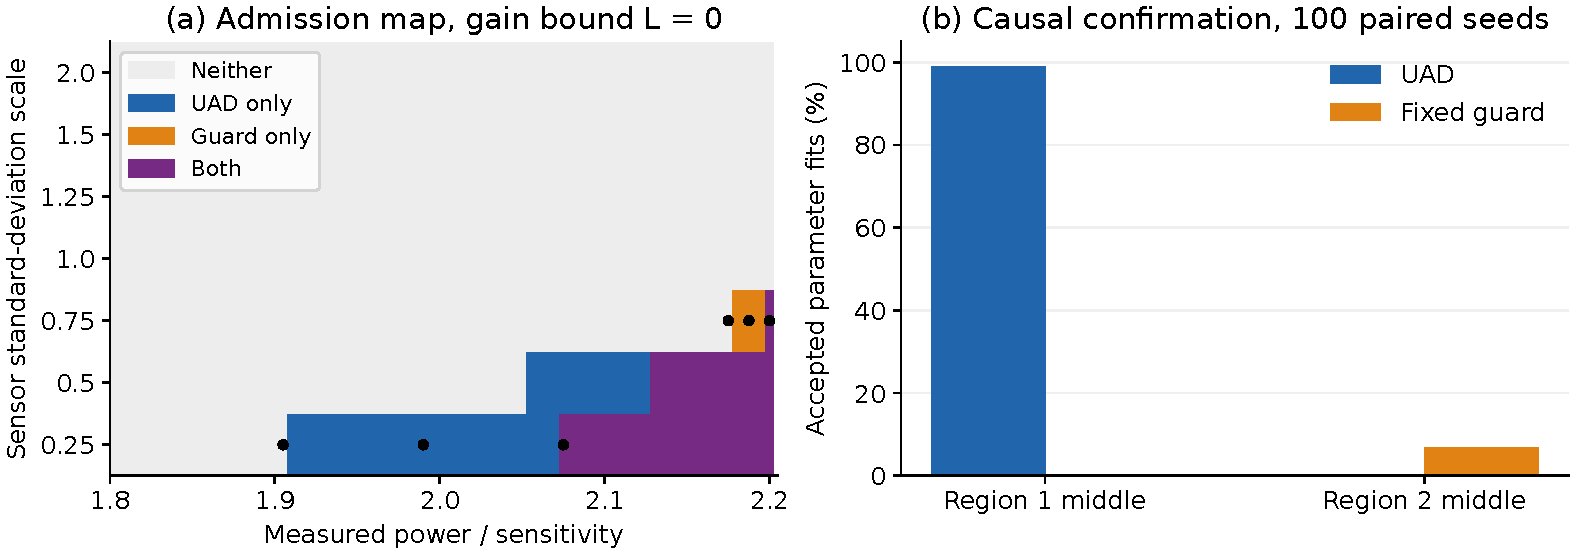
\includegraphics[width=\textwidth]{admission_confirmation.pdf}
\caption{Admission-map zoom at $\ell=0$ and causal midpoint confirmation. Dots mark all chosen controls and midpoints. The full 6,748-point map is supplied. Confirmation uses 100 paired seeds and all six fixed actuator members; percentages pool those declared members descriptively.}
\label{fig:frontier}
\end{figure*}

Seeds 7001--7100 are new. Each of six settings uses all six actual actuator pairs and two methods: 7,200 runs. The shared residual trigger requires three consecutive anomalies after warmup; no known fault time or label enters the decision. Gain changes at 2~s to the specified constant level; boresight offset is zero. The test concerns diagnosing attenuation on a usable link, not recovering an initially failed one. Nondeclining gain and reduced noise are stronger assumptions than the original affine-drift benchmark. Candidate dwells are 0.36~s and the excitation limit is 2.88~s for both methods.

\subsection{Complete records and independent replay}
Each run retains every standardized sensor disturbance, offset/gain history, full eight-state actuator trajectory, held reference, commanded and delivered torque, measured/actual power, candidate lower bound, premise checks, fit and outcome. Separate NumPy code reconstructs optical power, trigger, bounds, decisions and metrics, and replays every held-input RK4 step including stage clamping and anti-windup. Across 5,040,000 steps, maximum absolute state-step discrepancy is $3.39\times10^{-21}$ in the recorded state coordinates. It is independent calculation of the same model, not a physical replication.

Seed is the statistical unit. Within a seed, contrasts are averaged over the six fixed model pairs before 5,000 paired bootstrap resamples. Descriptive 95\% intervals and approximate Bonferroni percentile limits over six settings are supplied. Six model outputs from one seed are not six independent stochastic replicates. Historical V5 multiplicity reporting had an upper-percentile error: $.975/36$ was used instead of $1-.025/36$. Separate corrected exports preserve every per-run outcome and all ordinary 95\% endpoints, while changing 63 of 144 adjusted upper limits. V4's family-nine calculation was correct. The error and original records are retained transparently.

\begin{table*}[t]
\caption{Causal confirmation: each row has 100 seeds across six fixed actual models. Selection and acceptance are separate; confidence misses count accepted offsets outside their approximate radius. Slack is the median over selected traces of their median $(p-\underline p)/p_{\min}$. All settings have zero actual sampled outage. R1 and R2 are development-selected regions, not population categories.}
\centering\footnotesize
\begin{tabular}{llrrrrrr}\toprule
Setting & Method & Selected & Accepted fits & Outage (s) & Angular energy ($\mu$rad$^2$s) & Confidence misses & Slack\\\midrule
\FrontierRows
\bottomrule\end{tabular}
\label{tab:confirm}
\end{table*}

\section{Results and Evidence Categories}
In region~1's midpoint, UAD admits all 600 probes and accepts 594 parameter fits; the fixed guard admits none. Both have zero sampled outage. The paired acceptance-fraction difference is 0.990, with descriptive 95\% interval $[.970,1.000]$ over 100 seed units. This establishes diagnostic access under the stated finite-model, low-noise, nondeclining-gain conditions. It does not establish accurate diagnosis for every accepted fit or greater recovery speed. Six fits remain rejected; 26 of the 594 accepted offsets miss their approximate radius. The median accepted absolute gain error is $2.50\times10^{-4}$. The median trace-median bound slack is $0.658p_{\min}$, quantifying substantial residual conservatism rather than a tight power predictor.

The reverse direction matters. At region~2's midpoint, the fixed guard admits and accepts 41 probes while UAD refuses all. No guard run has observed sampled outage; these are not demonstrated unsafe admissions. The trigger selects the low part of the measurement distribution, so deterministic admission maps alone cannot predict causal admission rates. Surrounding controls in Table~\ref{tab:confirm} show this dependence. The original 2,800 identical V5 pairs and UAD's worse nominal recovery remain unchanged. For preserved affine drift, UAD has 5.0324~s mean outage and 46/50 acceptances versus DAP's 4.2420~s and 50/50.

Time-matched and native ES continue to answer different questions. Preserved 2.88-s ES affine-drift outage is 9.8404~s; native eight-second ES is 4.2676~s with much larger angular excitation. The tracker produces no verified diagnostic fit. Neither angular excitation nor probe authorization is an electrical-energy or diagnosis-success claim.

\begin{table}[t]
\caption{Strict UAD evidence categories for calculated bounds. Known failed premises take precedence; otherwise missing required histories mean unverified. Counts pool heterogeneous conditions descriptively, not as a field reliability estimate.}
\centering\footnotesize
\begin{tabular}{llrr}\toprule
Dataset & Evidence category & Probes & Bound failures\\\midrule
\EvidenceRows
\bottomrule\end{tabular}
\label{tab:evidence}
\end{table}

A \emph{within-premise} trace has the required histories and passes every numeric premise check under the declared simulator model. An \emph{out-of-model} trace has at least one established failed premise. An \emph{unverified} trace has no established failure but insufficient complete histories. These are evidence classes, not an inference that a noise distribution or physical calibration is proved by one trace.

V4's 1,564 reconstructed-compatible records are now strictly unverified because complete offset/rate-noise histories were not retained; the earlier labels remain unchanged. Its 557 known out-of-model probes include all 100 bound failures. V5 has complete offset/noise records; its strict categories are shown separately. V6 additionally has complete plant-state replay and 1,421 within-premise UAD probes with zero observed bound failures. The 204,624 shadow monitor samples show no observed breach. None of these selected, heterogeneous zero-event counts proves zero risk or a field failure target.

\FloatBarrier
\balance
\section{Interpretation, Limits, and Conclusion}
The exact property offered is a finite-mission, sampled-outage implication under explicit optical, sensor and finite-actuator hypotheses. Closest general AFD and safety-filtered ES methods establish different properties under their own assumptions; they are not declared deficient because their notation differs. Full optical mappings and faithful reproductions of those systems remain missing. Public Massa--Paulson code exists \cite{massacode}, but required CORA/solver functions were unavailable on the active MATLAB path. Exact overlap with recent optical acquisition work cannot be excluded without fuller source access. The result remains specialized, and absolute novelty is unconfirmed.

The new experiment identifies a limited use: a model-derived permission can provide diagnostic evidence where an overly large fixed guard refuses, without observed service loss in the tested usable-link regime. It also exposes the converse cost: a heuristic can acquire evidence while the certificate abstains, without observed failure. No test converts an inadequate guard into a theorem or conservative refusal into universally better operation. The prior identical-case result is therefore qualified by admission-frontier evidence, not deleted.

All physical parameters remain assumptions. Independent actuator replay, optical quadrature and algebra validate calculations of the declared simulation model. They do not establish a calibrated receiver, real actuator uncertainty, industrial integration, hardware-in-the-loop behavior or flight readiness. Continuous inertia/lag intervals, abrupt offset changes during a probe, heavy tails, sensor bias and post-probe correction safety remain outside the proved statement. An operational supervisor must refuse unsupported contracts rather than hide them behind a scalar ``safe'' flag.

The defensible contribution is conditional probe authorization with a verified scope, a measurable but restricted diagnostic-admission difference, transparent incomplete-evidence categories and executable supervisory refusal logic. Physical validation, external mathematical review, stronger original-paper comparisons and source-rights/human-author approvals remain open. This is a research revision, not a claim of readiness for IEEE Transactions on Industrial Informatics or another Transactions venue.

\section*{Reproducibility and Assistance}
V4 and V5 are preserved with hash records. Supplementary sources include the full map, frozen confirmation protocol, complete new traces, replay/checker code, corrected statistical exports, evidence categories and supervisory tests. The original terminal model is reused and attributed \cite{source}. OpenAI Codex assisted formulation, implementation, verification calculations, literature review, figures and drafting. Recorded MATLAB runs generated the plant results; no independent human review is invented. Substantive assistance is disclosed consistently with IEEE guidance \cite{aipolicy}.
\begin{thebibliography}{99}
\bibitem{guelman} M. Guelman \emph{et al.}, ``Acquisition and pointing control for inter-satellite laser communications,'' \emph{IEEE Transactions on Aerospace and Electronic Systems}, vol. 40, no. 4, pp. 1239--1248, 2004, doi: \href{https://doi.org/10.1109/TAES.2004.1386877}{\nolinkurl{10.1109/TAES.2004.1386877}}.
\bibitem{es} M. Krstić, H. Wang, ``Stability of extremum seeking feedback for general nonlinear dynamic systems,'' \emph{Automatica}, vol. 36, no. 4, pp. 595--601, 2000, doi: \href{https://doi.org/10.1016/S0005-1098(99)00183-1}{\nolinkurl{10.1016/S0005-1098(99)00183-1}}.
\bibitem{guo} Y. Guo, Q. Liu, Z. Wang, Z. Zhang \emph{et al.}, ``Active fault diagnosis for linear stochastic systems subject to chance constraints,'' \emph{Automatica}, vol. 156, Art. no. 111194, 2023, doi: \href{https://doi.org/10.1016/j.automatica.2023.111194}{\nolinkurl{10.1016/j.automatica.2023.111194}}.
\bibitem{massa} N. Massa, J. A. Paulson, ``Optimal input design for guaranteed fault diagnosis of nonlinear systems: An active deep learning approach,'' \emph{Control Engineering Practice}, vol. 153, Art. no. 106118, 2024, doi: \href{https://doi.org/10.1016/j.conengprac.2024.106118}{\nolinkurl{10.1016/j.conengprac.2024.106118}}.
\bibitem{safees} A. Williams, M. Krstic, A. Scheinker, ``Semiglobal Safety-Filtered Extremum Seeking With Unknown CBFs,'' \emph{IEEE Transactions on Automatic Control}, vol. 70, no. 3, pp. 1698--1713, 2025, doi: \href{https://doi.org/10.1109/TAC.2024.3469785}{\nolinkurl{10.1109/TAC.2024.3469785}}.
\bibitem{yan} K. Yan, B. Guo, Y. Zhou, X. Xue \emph{et al.}, ``Link-Margin-Aware joint parameter optimization for scanning and acquisition of optical inter-satellite link,'' \emph{Optics Communications}, vol. 616, Art. no. 133342, 2026, doi: \href{https://doi.org/10.1016/j.optcom.2026.133342}{\nolinkurl{10.1016/j.optcom.2026.133342}}.
\bibitem{source} Satellite-Optical-Fault-Recovery, source terminal model and V2 implementation, local archived snapshot \texttt{0bc453ffa0ad}. \href{https://github.com/kaushalrog/Satellite-Optical-Fault-Recovery}{Source repository}; accessed Oct. 23, 2026.
\bibitem{actuators} M. Milaševičius, L. Mačiulis, ``A Review of Mechanical Fine-Pointing Actuators for Free-Space Optical Communication,'' \emph{Aerospace}, vol. 11, no. 1, Art. no. 5, 2024, doi: \href{https://doi.org/10.3390/aerospace11010005}{\nolinkurl{10.3390/aerospace11010005}}.
\bibitem{baeck} K. Baeck, J. Wi, H. Yoon, ``Analytic pointing error evaluation on nano-satellite laser communication system,'' \emph{Optics Communications}, vol. 559, Art. no. 130419, 2024, doi: \href{https://doi.org/10.1016/j.optcom.2024.130419}{\nolinkurl{10.1016/j.optcom.2024.130419}}.
\bibitem{nasa} NASA Small Spacecraft Systems Virtual Institute, ``State-of-the-art small spacecraft technology: Communications.'' \href{https://www.nasa.gov/smallsat-institute/sst-soa/soa-communications/}{NASA communications overview}; accessed Oct. 23, 2026.
\bibitem{massacode} Paulson Laboratory, ``Guaranteed\_AFD\_ADL: Author implementation,'' accessed Oct. 23, 2026. [Online]. Available: \url{https://github.com/PaulsonLab/Guaranteed_AFD_ADL}
\bibitem{aipolicy} IEEE Author Center, ``Submission and peer review policies: Use of AI by authors.'' \href{https://journals.ieeeauthorcenter.ieee.org/become-an-ieee-journal-author/publishing-ethics/guidelines-and-policies/submission-and-peer-review-policies/}{IEEE policy}; accessed Oct. 23, 2026.
\end{thebibliography}

\end{document}
